% Generated by Listas/make_statements.py from pratica-lecture-03.md, item 3. Do not edit.
\textbf{Source.} Muñoz-Garcia \& Toro-Gonzalez (2019), \emph{Strategy and Game Theory: Practice Exercises with Answers}, Ch. 4, Exercise 3 ``Sequential Version of the Prisoner's Dilemma Game'', p.~160 {[}PDF 172{]}. Reproduced verbatim (statement only; the book's worked answer follows it).



\begin{quote}

Consider the game tree in Fig. 4.9, representing the sequential-move version of the Prisoner's dilemma game, where player 1 acts first, and observing its move player 2 responds.



\pandocbounded{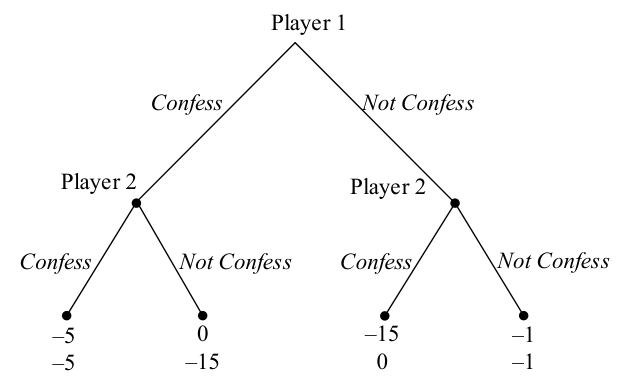
\includegraphics[keepaspectratio,alt={Fig. 4.9 Prisoner's dilemma sequential-move game}]{../figures/munoz-garcia-4-3.png}}



\emph{Fig. 4.9} Prisoner's dilemma sequential-move game



\begin{enumerate}

\def\labelenumi{(\alph{enumi})}

\item

  Find the best responses of the second mover, for each of the first mover's actions.

\item

  Find the first mover's equilibrium action and describe the subgame perfect Nash equilibrium of the game.

\item

  Does the equilibrium behavior in the sequential-move game differ from its simultaneous-move version?

\end{enumerate}

\end{quote}

